% Prarup: final project report. Layout modelled on the Hagenberg Thesis class
% (hgbthesis, W. Burger and W. Hochleitner, CC-BY-4.0), rebuilt for XeTeX.
\documentclass[11pt,a4paper,oneside,openany]{book}
\usepackage[a4paper,top=30mm,bottom=30mm,inner=30mm,outer=25mm,headsep=10mm]{geometry}
\usepackage{fontspec}
\newfontfamily\deva{Kohinoor Devanagari}[Script=Devanagari]
\usepackage{amsmath}
\usepackage{xcolor}
\definecolor{dau}{RGB}{38,47,133}
\definecolor{dauorange}{RGB}{232,89,12}
\definecolor{dauyellow}{RGB}{245,180,0}
\definecolor{ink}{RGB}{30,30,30}
\definecolor{soft}{RGB}{246,246,250}
\definecolor{rule}{RGB}{200,200,210}
\usepackage{graphicx}
\usepackage{booktabs,tabularx,array,longtable,multirow}
\usepackage{enumitem}
\usepackage{caption}
\captionsetup{font=small,labelfont={bf,sf},format=hang}
\usepackage{titlesec}
\usepackage{fancyhdr}
\usepackage{tikz}
\usetikzlibrary{arrows.meta,positioning,fit,backgrounds,calc,shapes.geometric}
\usepackage{pgfplots}
\pgfplotsset{compat=1.17}
\usepackage{listings}
\usepackage{microtype}
\usepackage[colorlinks=true,linkcolor=dau,urlcolor=dau,citecolor=dau]{hyperref}
\usepackage{setspace}
\setstretch{1.12}
\setlist{itemsep=0.15em,topsep=0.3em}
\setlength{\parskip}{0.35em}
\raggedbottom

% Hagenberg-style headings: sans serif, number set apart
\titleformat{\chapter}[display]{\sffamily\bfseries\color{dau}}
  {\Large\chaptertitlename\ \thechapter}{0.6em}{\huge}
\titlespacing*{\chapter}{0pt}{0pt}{28pt}
\titleformat{\section}{\sffamily\bfseries\Large\color{dau}}{\thesection}{0.8em}{}
\titleformat{\subsection}{\sffamily\bfseries\large}{\thesubsection}{0.8em}{}
\titleformat{\paragraph}[runin]{\sffamily\bfseries}{}{0pt}{}[.]
\pagestyle{fancy}
\fancyhf{}
\renewcommand{\headrulewidth}{0.3pt}
\fancyhead[L]{\small\sffamily\leftmark}
\fancyhead[R]{\small\sffamily\thepage}
\renewcommand{\chaptermark}[1]{\markboth{\thechapter.\ #1}{}}
\fancypagestyle{plain}{\fancyhf{}\renewcommand{\headrulewidth}{0pt}\fancyfoot[C]{\small\sffamily\thepage}}

\lstset{basicstyle=\ttfamily\small,columns=fullflexible,keepspaces=true,breaklines=true,
  frame=single,rulecolor=\color{rule},backgroundcolor=\color{soft},language=Python,
  keywordstyle=\color{dau}\bfseries,commentstyle=\color{gray}\itshape,showstringspaces=false}

\newcommand{\code}[1]{\texttt{#1}}
\usepackage[most]{tcolorbox}
\newtcolorbox{takeaway}{enhanced, blanker, borderline west={2.5pt}{0pt}{dauorange},
  left=10pt, top=3pt, bottom=3pt, before skip=8pt, after skip=10pt,
  fontupper=\sffamily\small\color{ink}}

\tikzset{
  blk/.style={draw=dau!70,fill=dau!6,rounded corners=2pt,align=center,font=\small\sffamily,inner sep=5pt,minimum height=9mm},
  hot/.style={draw=dauorange!80,fill=dauorange!8,rounded corners=2pt,align=center,font=\small\sffamily,inner sep=5pt,minimum height=9mm},
  ext/.style={draw=gray!60,fill=gray!8,rounded corners=2pt,align=center,font=\small\sffamily,inner sep=4pt},
  arr/.style={-{Stealth[length=2.2mm]},thick,dau!80},
  lab/.style={font=\scriptsize\sffamily,text=dauorange!90!black,fill=white,inner sep=1pt}}

\begin{document}

% ---------------------------------------------------------------- title page
\begin{titlepage}
\centering

\includegraphics[width=0.45\textwidth]{dau-logo.jpg}\par
\vspace{18mm}
{\sffamily\bfseries\Huge\color{dau} Prarup\par}
\vspace{3mm}
{\large\deva प्रारूप\par}
\vspace{8mm}
{\sffamily\Large An offline desktop tool that turns a research paper\\ into a checked IEEE conference paper\par}
\vspace{16mm}
{\large\textsc{Final Project Report}\par}
\vspace{4mm}
{\normalsize PC503 \textperiodcentered{} Programming with Python\par}
\vfill
\begin{tabular}{l l}
Prateek Kalal & 202611009\\
Om Patel & 202611030\\
Krushna Parmar & 202611032\\
\end{tabular}
\vspace{14mm}

{\sffamily Dhirubhai Ambani University, Gandhinagar\par}
{\sffamily November 2026\par}
\end{titlepage}

\frontmatter
\chapter*{Abstract}
\addcontentsline{toc}{chapter}{Abstract}
Many conference papers are turned away before a reviewer reads them, for faults the author cannot see:
fonts that were never embedded in a figure, figures wider than their column, a missing abstract or caption,
a citation that points at nothing. The author usually learns this on the day of the deadline, from a
validator that replies with a failure and little else. Prarup moves that verdict to a point where the
author can still act on it. It opens a paper written in Word or \LaTeX, shows it as a tagged outline,
lists everything that is missing or wrong, lets the author fix each item in place, and builds the IEEE
conference PDF, which it then inspects the way IEEE PDF eXpress does. It also measures every figure on
the printed page and resizes figures until their text is readable, and it reports evidence that an image
was produced by a generative model, from signed provenance records down to an optional classifier.
Everything runs on the author's own computer. We tested Prarup on six real papers, three of which are
openly licensed and included with the code, and on deliberately damaged copies of them. Before our
redesign only two of five real papers compiled; after it, all six compile, and every planted fault is
detected and can be repaired through the window. The code is 3{,}663 lines of Python, covered by 147
automated tests.

\chapter*{How to read this report}
\addcontentsline{toc}{chapter}{How to read this report}
The report is written so that a reader who stops after any chapter still leaves with a correct, if
incomplete, picture of the system. Chapter~\ref{ch:model} gives that picture first: one diagram and four
ideas that explain almost every design choice. Each later chapter adds detail to one part of the picture,
and opens with a short statement of its point, in a ruled box, before the evidence.

Three writing guides shaped this structure. Minto's pyramid principle puts the answer before the
reasoning~\cite{minto}. Gopen and Swan's study of how readers process scientific prose asks that each
sentence begin with familiar information and end with the new point~\cite{gopen}. Pinker's ``classic
style'' treats the reader as an intelligent equal who should be shown, not told~\cite{pinker}. Where we
report a number, it was measured on a real run, and the run is described in Chapter~\ref{ch:eval}.

\tableofcontents

\mainmatter

% ---------------------------------------------------------------- 1
\chapter{Introduction}\label{ch:intro}

\begin{takeaway}
Formatting faults, not research quality, sink many submissions, and the faults that matter most are
invisible in the author's own view of the paper. Prarup finds them before submission and fixes the ones
that can be fixed.
\end{takeaway}

\section{The problem}
A conference paper passes through two gates. The first is a reviewer who judges the research. The second,
which comes earlier, is a mechanical check of the file. IEEE asks every author to run the PDF through its
PDF eXpress service, which rejects files with fonts that are not embedded, with bitmap (Type~3) fonts, with
security settings, and with other defects~\cite{pdfexpress}. The most common cause is not the author's text
at all. Plotting libraries such as matplotlib export charts that reference a font, usually Helvetica,
without including it. Nothing on screen reveals this, nothing appears in the \LaTeX{} log, and the
validator's report does not say which figure is to blame.

Other faults are visible but easy to miss under deadline pressure: a figure without a caption, an abstract
lost when a Word template was changed, a reference list that ends at 50 entries while the text cites
[99], a chart whose axis labels print at four points. Each one is small. Together they cost authors days
of formatting work that a program could do in seconds.

\section{What Prarup does}
Prarup is a desktop application that takes a manuscript in either of the two formats researchers actually
use, Word (\code{.docx}) or \LaTeX{} (a \code{.tex} file or a zipped project), and does five things:
\begin{enumerate}
\item \textbf{Reads the paper into a structure} the author can see: every block tagged as a title, author,
abstract, heading, paragraph, figure, table, equation or reference list.
\item \textbf{Lists what is missing or wrong}, from a missing abstract to a citation past the end of the
references, and opens the right block when the author clicks a problem.
\item \textbf{Checks every image}: its resolution when printed, whether it duplicates another figure, and
whether there is evidence it was made by a generative model.
\item \textbf{Builds the IEEE conference PDF} a moment after each edit, and inspects it: fonts, page limit,
encryption, bookmarks, figures that run past their column, figure text too small to read.
\item \textbf{Repairs what can be repaired}: it embeds missing fonts, resizes figures until their text
reaches 7~pt, and exports a submission archive with a report of every check.
\end{enumerate}

\section{Contributions}
Beyond packaging existing tools, the project makes four contributions that we could not find together in
any single tool we surveyed:
\begin{itemize}
\item \textbf{One editable structure for both input formats}, so the same outline, editors and checks work
for Word and \LaTeX{} papers.
\item \textbf{Figure measurement on the compiled page}, using invisible PDF links as markers, which lets the
program state the printed size of a figure's text in points and resize the figure to a target.
\item \textbf{Layered, honest AI-image evidence}, which separates signed proof of origin from traces and
from a statistical guess, and refuses to run the guess on charts after we measured its false alarms there.
\item \textbf{A test bed of real and deliberately damaged papers}, so every claim in this report can be
re-run.
\end{itemize}

% ---------------------------------------------------------------- 2
\chapter{A mental model of Prarup}\label{ch:model}

\begin{takeaway}
Think of Prarup as a loop around one object, the \emph{manuscript}. The paper is read into it once; checks
look at it; the author edits it; and the PDF is rebuilt from it after every edit. Four ideas explain almost
every design choice.
\end{takeaway}

\begin{figure}[htbp]
\centering
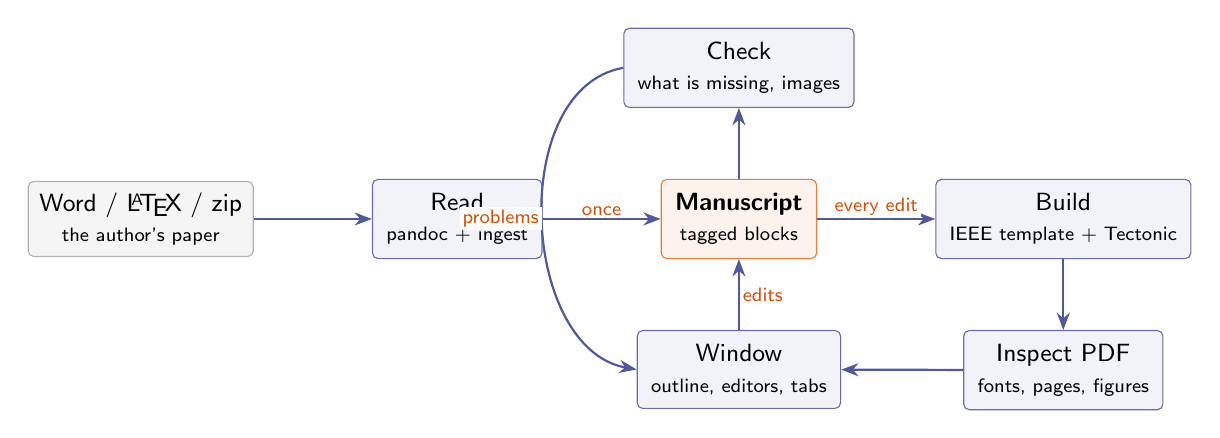
\begin{tikzpicture}[node distance=9mm and 15mm]
\node[ext] (paper) {Word / \LaTeX{} / zip\\\scriptsize the author's paper};
\node[blk, right=of paper] (read) {Read\\\scriptsize pandoc + ingest};
\node[hot, right=of read] (m) {\textbf{Manuscript}\\\scriptsize tagged blocks};
\node[blk, above=of m] (check) {Check\\\scriptsize what is missing, images};
\node[blk, right=of m] (build) {Build\\\scriptsize IEEE template + Tectonic};
\node[blk, below=of build] (inspect) {Inspect PDF\\\scriptsize fonts, pages, figures};
\node[blk, below=of m] (window) {Window\\\scriptsize outline, editors, tabs};
\draw[arr] (paper) -- (read);
\draw[arr] (read) -- node[lab,above]{once} (m);
\draw[arr] (m) -- (check);
\draw[arr] (check.west) to[out=190,in=170] node[lab,left]{problems} (window.west);
\draw[arr] (window) -- node[lab,right]{edits} (m);
\draw[arr] (m) -- node[lab,above]{every edit} (build);
\draw[arr] (build) -- (inspect);
\draw[arr] (inspect) -- (window);
\end{tikzpicture}
\caption{The whole program. The manuscript sits in the middle; everything else reads it or changes it.}
\label{fig:loop}
\end{figure}

\section{Four ideas}

\paragraph{One structure for every input}
Word and \LaTeX{} papers are both converted by pandoc~\cite{pandoc} into the same tree, and from that into
our own \code{Manuscript} of tagged \code{Block}s. After this step nothing in the program knows or cares which
format the paper came from. One editor, one set of checks and one renderer serve both.

\paragraph{Rebuild, do not copy}
Prarup does not try to compile the author's own \LaTeX{}. It writes the paper again into its own IEEE
template, carrying over only the author's mathematical packages and macros. This sounds wasteful but it is
what made real papers work: every Word table that pandoc writes as a \code{longtable} is illegal in a
two-column paper, and arXiv papers written for pdf\LaTeX{} load packages that a modern engine rejects.

\paragraph{Measure, do not guess}
Every check gives a fixed answer computed from the file: whether a font is embedded is read from the PDF;
the printed size of a figure's text is measured on the compiled page. No language model decides whether a
paper is compliant.

\paragraph{Evidence, not verdicts}
Where certainty is impossible, as with AI-generated images, Prarup reports the evidence and its strength,
and says what absence of evidence means. A signed provenance record is reported as an error; a classifier
score is reported as a likelihood and never run where we measured it to be unreliable.

\section{Who built which part}
The work divides along the same lines as Figure~\ref{fig:loop}. Each member owns between 1{,}195 and
1{,}242 lines of code and the tests for them (Table~\ref{tab:roles}).

\begin{table}[htbp]
\centering\small
\caption{Ownership of the code. Line counts exclude tests and the template.}
\label{tab:roles}
\begin{tabularx}{\linewidth}{>{\bfseries}l X r}
\toprule
Member & Responsibility and files & Lines\\
\midrule
Prateek Kalal & Reading the paper and checking its images: \code{ingest}, \code{frontmatter}, \code{pandoc}, \code{texsource}, \code{manuscript}, \code{images} & 1{,}195\\
Krushna Parmar & Building the IEEE PDF and checking it: \code{analyze}, \code{renderer}, \code{compile}, \code{figures}, \code{measure}, \code{checks}, \code{fit}, \code{fix}, \code{models} & 1{,}226\\
Om Patel & The Tkinter window and the controller that joins everything: \code{project}, \code{main}, \code{process}, \code{ui/*} & 1{,}242\\
\bottomrule
\end{tabularx}
\end{table}

% ---------------------------------------------------------------- 3
\chapter{Background}\label{ch:bg}

\begin{takeaway}
Prarup stands on four well-tested tools and one standard. Knowing what each does explains where our own
code begins.
\end{takeaway}

\section{What IEEE checks}
IEEE conferences ask for the \code{IEEEtran} two-column layout and a PDF that passes PDF eXpress. The checks
that matter most for this project are: every font embedded, no Type~3 bitmap fonts, no encryption, the page
limit respected, and figures and tables kept within the page geometry~\cite{pdfexpress,ieeetran}. IEEE also
asks for images of at least 300 dots per inch at their printed size~\cite{ieeegraphics}.

\section{The tools we build on}
\begin{description}[style=nextline,leftmargin=2em]
\item[pandoc] A document converter that reads Word and \LaTeX{} into a common tree of typed nodes, and writes
that tree back out as Markdown or \LaTeX~\cite{pandoc}. It is the reason one program can read both formats.
\item[Tectonic] A self-contained \LaTeX{} engine that downloads the packages a document needs on first use,
so a user does not have to install a full \TeX{} distribution~\cite{tectonic}.
\item[PyMuPDF] A Python library for reading PDF files: fonts per page, text with its size and position,
image rectangles, links, and page rendering~\cite{pymupdf}.
\item[Ghostscript and Tesseract] Ghostscript rewrites a PDF with every font embedded~\cite{ghostscript};
Tesseract recognises words in an image and reports each word's box~\cite{tesseract}.
\end{description}

\section{Provenance of images}
The Coalition for Content Provenance and Authenticity (C2PA) defines a signed manifest that an image
generator attaches to its output, recording how the image was made~\cite{c2pa}. IPTC defines a
``digital source type'' vocabulary in which \code{trainedAlgorithmicMedia} means an image produced by a
trained model~\cite{iptc}. Google's Gemini, for example, signs its images with both. When this metadata
has been removed, only statistical detection remains, and such detectors are known to be unreliable outside
the kind of images they were trained on.

\section{Related tools}
PDF eXpress itself reports faults but neither locates the guilty figure nor fixes it. Overleaf and other
\LaTeX{} editors compile papers but do not check them against a conference's rules, and do not open Word
files. Word's own templates format text but cannot see inside figures. Prarup's niche is the gap between
these: one offline tool that reads both formats, checks what the validator checks, and repairs what it can.

% ---------------------------------------------------------------- 4
\chapter{Design}\label{ch:design}

\begin{takeaway}
The program has three layers that talk only downwards: the window, a controller, and the modules that do
the work. Every outside program is reached through one small function. This keeps each file about one
thing, which made the code easy to test and to explain.
\end{takeaway}

\section{Architecture}

\begin{figure}[htbp]
\centering
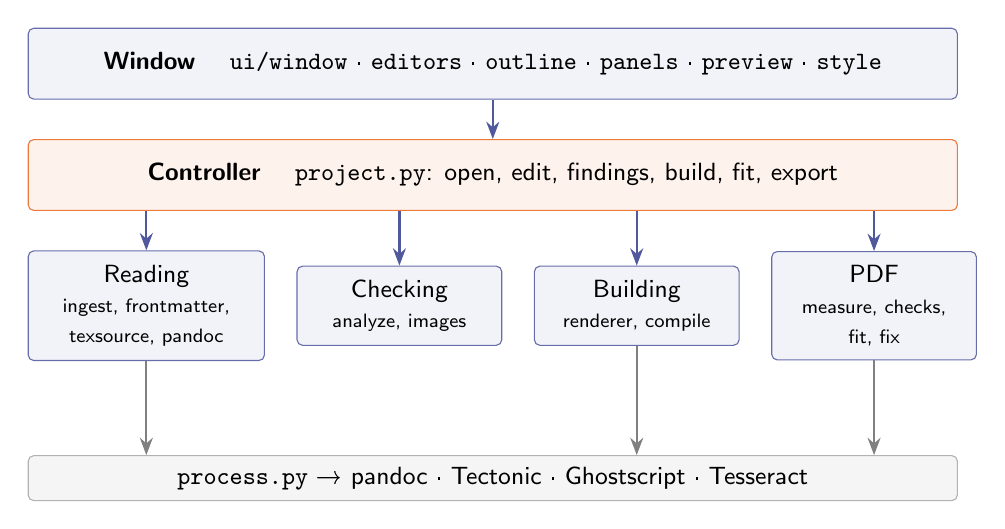
\begin{tikzpicture}[node distance=5mm and 4mm]
\node[blk, minimum width=118mm] (ui) {\textbf{Window} \quad \code{ui/window} \textperiodcentered{} \code{editors} \textperiodcentered{} \code{outline} \textperiodcentered{} \code{panels} \textperiodcentered{} \code{preview} \textperiodcentered{} \code{style}};
\node[hot, below=of ui, minimum width=118mm] (proj) {\textbf{Controller} \quad \code{project.py}: open, edit, findings, build, fit, export};
\node[blk, below=of proj, xshift=-44mm, minimum width=30mm] (rd) {Reading\\\scriptsize ingest, frontmatter,\\\scriptsize texsource, pandoc};
\node[blk, right=of rd, minimum width=26mm] (ck) {Checking\\\scriptsize analyze, images};
\node[blk, right=of ck, minimum width=26mm] (bd) {Building\\\scriptsize renderer, compile};
\node[blk, right=of bd, minimum width=26mm] (pd) {PDF\\\scriptsize measure, checks,\\\scriptsize fit, fix};
\node[ext, below=of proj, yshift=-26mm, minimum width=118mm] (ex) {\code{process.py} \textrightarrow{} pandoc \textperiodcentered{} Tectonic \textperiodcentered{} Ghostscript \textperiodcentered{} Tesseract};
\draw[arr] (ui) -- (proj);
\foreach \n in {rd,ck,bd,pd} \draw[arr] (proj.south -| \n.north) -- (\n.north);
\foreach \n in {rd,bd,pd} \draw[arr,gray] (\n.south) -- (\n.south |- ex.north);
\end{tikzpicture}
\caption{Three layers. The window never reads a paper or a PDF itself; the modules never touch a widget.}
\label{fig:arch}
\end{figure}

The controller, \code{Project}, is a facade: the window calls one method such as \code{build()}, and the
controller performs the steps behind it in order (render, instrument, compile, measure, strip markers,
check). Every edit method saves the manuscript to \code{manuscript.json} at once, so no work is lost if the
program closes, and reopening a paper restores the author's edits unless the source file has changed since.

\section{The data model}
Two dataclasses carry the paper through the program. A \code{Manuscript} holds the title, authors, abstract,
keywords, notes made while reading, and a list of \code{Block}s. A \code{Block} has an identifier, a kind,
its text in Markdown, and the fields its kind needs: images, caption and fitted width for figures, entries
and citation keys for references. Each block also keeps the original pandoc node, because some things,
such as table cells, cannot be rebuilt from text alone.

\begin{figure}[htbp]
\centering
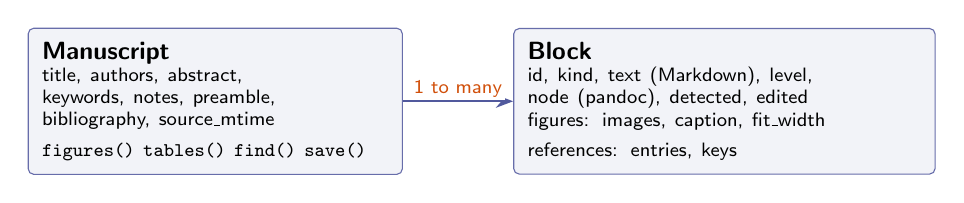
\begin{tikzpicture}[node distance=6mm and 14mm]
\node[blk, text width=44mm, align=left] (m) {\textbf{Manuscript}\\\scriptsize title, authors, abstract,\\\scriptsize keywords, notes, preamble,\\\scriptsize bibliography, source\_mtime\\\scriptsize \code{figures()} \code{tables()} \code{find()} \code{save()}};
\node[blk, right=of m, text width=50mm, align=left] (b) {\textbf{Block}\\\scriptsize id, kind, text (Markdown), level,\\\scriptsize node (pandoc), detected, edited\\\scriptsize figures: images, caption, fit\_width\\\scriptsize references: entries, keys};
\draw[arr] (m) -- node[lab,above]{1 to many} (b);
\end{tikzpicture}
\caption{The two classes every part of the program shares.}
\end{figure}

\section{Design decisions}

\begin{table}[htbp]
\centering\small
\caption{The decisions that shaped the program, with the alternatives we rejected.}
\begin{tabularx}{\linewidth}{>{\raggedright\arraybackslash}p{30mm} >{\raggedright\arraybackslash}X >{\raggedright\arraybackslash}X}
\toprule
Decision & Alternative considered & Why we chose it\\
\midrule
Rebuild the paper in our own template & Compile the author's \LaTeX{} as it is & Real papers failed on \code{longtable} and pdf\LaTeX-only packages; rebuilding made 6 of 6 compile\\
pandoc for both formats & Separate parsers for Word and \LaTeX & One tree, one code path; months of parsing work avoided\\
Markdown as the internal text format & Keep pandoc nodes only & Authors can read and edit Markdown in a plain text box\\
Tkinter for the window & PySide6 (our first version), a web UI & Ships with Python, simple enough to explain line by line; a desktop app was required\\
One background thread & Run jobs on the window's thread & The window must not freeze during a 3 to 10 second build\\
Rules in a YAML file & Numbers in the code & Another conference needs a new file, not new code\\
Classifier only on photos & Run it on every image & We measured 4 false alarms on 26 real charts\\
\bottomrule
\end{tabularx}
\end{table}

\section{Design principles in the code}
The layering follows from separation of concerns, and the SOLID principles appear in specific places.
Each outside program is started by exactly one function (single responsibility); a test fails if the PDF
checks ever import \code{subprocess} or \code{tkinter}. A new kind of block needs a new editor class and one
line in the factory \code{editor\_for} (open/closed). The window calls \code{save()} on whichever editor it
holds, and every editor keeps the same contract (Liskov substitution). The outline and the tabs receive a
single callback function rather than the whole window (interface segregation, dependency inversion). We
also note where the code bends these rules: the main window both lays out widgets and handles every
action, which a larger project would split.

% ---------------------------------------------------------------- 5
\chapter{Implementation}\label{ch:impl}

\begin{takeaway}
This chapter follows a paper through the program in the order of Figure~\ref{fig:loop}: read, check,
build, inspect, fit, and finally the window that ties them together.
\end{takeaway}

\section{Reading a paper}
\code{ingest.open\_paper} unpacks a zip safely (refusing any entry whose path would escape the target
folder), asks pandoc for the document tree, and removes wrapper nodes so the blocks form one flat list. It
then finds the title block and tags each remaining block. Real Word papers rarely use proper styles, so
most of this code is a set of patterns learned from the papers we tested (Table~\ref{tab:patterns}).

\begin{table}[htbp]
\centering\small
\caption{Patterns found in real Word papers and how Prarup handles them.}
\label{tab:patterns}
\begin{tabularx}{\linewidth}{>{\raggedright\arraybackslash}X >{\raggedright\arraybackslash}X}
\toprule
Pattern as found & Handled as\\
\midrule
Abstract and keywords inside a layout table, spelt ``A B S T R A C T'' & read out of the table, letters joined\\
No heading styles; sections as short bold paragraphs & headings, marked as detected\\
``Introduction:'' as a plain line & heading\\
Caption as its own paragraph after the image, or as a quote & joined to the figure; ``Figure 2:'' removed\\
Superscript-numbered affiliations & each author gets their numbered affiliation\\
A caption whose image did not survive conversion & a figure with no image, reported\\
Inline maths followed by ``(2)'' & an equation\\
\bottomrule
\end{tabularx}
\end{table}

For \LaTeX{} papers, pandoc loses IEEE author blocks, \code{\textbackslash bibitem} lists and the author's
macros, so \code{texsource.py} reads these directly from the source with small parsers that count braces.
Only safe packages are carried over (mathematics, algorithms, tables), and every \code{\textbackslash newcommand}
becomes \code{\textbackslash providecommand}, so a clash with our template cannot stop the build.

Conversion to Markdown is batched. Starting pandoc costs time, so all paragraphs are joined with a marker
word, converted in one run, and split again; a paper with hundreds of blocks needs three runs, not hundreds.

\section{Finding what is missing}
\code{analyze.py} examines the manuscript before anything is compiled and returns a list of findings, each
with a code, a severity and the block it belongs to (Table~\ref{tab:codes}). Clicking a finding in the
window opens that block.

\begin{table}[htbp]
\centering\small
\caption{Manuscript findings.}
\label{tab:codes}
\begin{tabularx}{\linewidth}{l X l}
\toprule
Code & Finding & Severity\\
\midrule
META-01 to 04 & No title; no authors or affiliation; no abstract; no keywords & error / warning\\
FIG-01 to 04 & No caption; never mentioned; no image or missing file; unusable format & warning / error\\
TAB-01, 02 & No caption; never mentioned & warning\\
REF-01 to 03 & No references; citation without a reference; reference never cited & error / warning\\
STR-01, 02 & No Introduction or Conclusion; an empty section & warning\\
\bottomrule
\end{tabularx}
\end{table}

Citations are checked in two ways. When citation keys are known (from a \code{.bib} file or
\code{\textbackslash bibitem}s), the set of cited keys is compared with the set of reference keys. When
references are numbered, any cited number larger than the number of entries is an error; this is how a
planted ``[99]'' in a paper with 50 references is caught.

\section{Checking images}
Every figure image is checked for its printed resolution (pixels divided by printed width in inches,
assuming the IEEE column of 3.5~in when no measurement exists), for duplicates, and for AI evidence in
three layers (Figure~\ref{fig:layers}). Duplicates are found with a 64-bit difference hash~\cite{dhash}:
two images whose hashes differ in at most four bits are the same picture, which survives resizing and
recompression.

\begin{figure}[htbp]
\centering
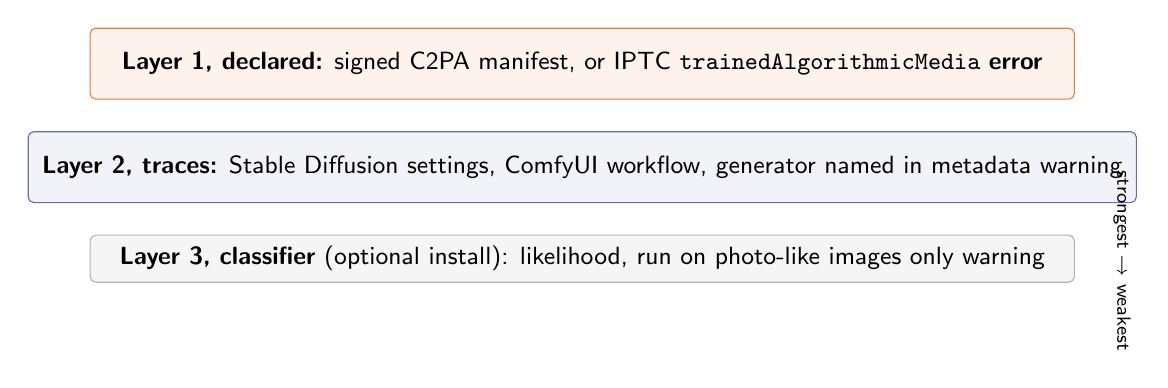
\begin{tikzpicture}[node distance=4mm]
\node[hot, minimum width=125mm] (l1) {\textbf{Layer 1, declared:} signed C2PA manifest, or IPTC \code{trainedAlgorithmicMedia} \hfill \textbf{error}};
\node[blk, below=of l1, minimum width=125mm] (l2) {\textbf{Layer 2, traces:} Stable Diffusion settings, ComfyUI workflow, generator named in metadata \hfill warning};
\node[ext, below=of l2, minimum width=125mm] (l3) {\textbf{Layer 3, classifier} (optional install): likelihood, run on photo-like images only \hfill warning};
\node[font=\scriptsize\sffamily, right=2mm of l1.east, anchor=west, rotate=-90, yshift=4mm] at ($(l1.east)!0.5!(l3.east)$) {strongest \textrightarrow{} weakest};
\end{tikzpicture}
\caption{AI evidence is reported in order of strength, and only the strongest layer found is reported.}
\label{fig:layers}
\end{figure}

The classifier~\cite{aiclassifier} is a trained model that outputs a probability. When we ran it on the 26
bitmap figures of five real papers, it scored four charts and logos between 0.85 and 1.00, which would have
accused honest authors. We therefore separate photographs from charts by colour: a chart's eight most common
colours cover at least 90\% of its pixels (we measured 0.94 to 1.00 for charts and 0.47 to 0.89 for photos
and generated art), and the classifier runs only on the second group.

\section{Building the IEEE PDF}
\code{renderer.py} writes the manuscript into an IEEE template using Jinja2. Because \LaTeX{} uses braces
everywhere, the template markers are changed to \code{\textbackslash VAR\{\}} and \code{\textbackslash BLOCK\{\}}.
Paragraphs the author has not edited are written from their original pandoc nodes, which lose nothing;
edited ones are converted from Markdown. Tables are written by our own code: the natural width of a table
is estimated from the longest text in each column, and a table wider than 1.6 columns spans both. Missing
images become a framed ``image missing'' box, so the paper always builds and the gap is visible. Tectonic
then compiles the result; the previous PDF is deleted first, so a failed build can never be checked by
mistake against an old file.

\section{Inspecting the PDF}
\code{checks.py} reads the compiled PDF with PyMuPDF: the fonts on each page (a font whose file is listed as
``n/a'' is not embedded; a Type~3 font is a bitmap font), the page count, encryption, bookmarks, and every
image's rectangle compared with the column it belongs to. The column geometry is not hard-coded; the
template writes the real column width, text width, margin and gap into the PDF's information dictionary
while compiling, and the checks read them back. Faults that Ghostscript can repair (missing fonts,
encryption) are marked so the Fix PDF button can rewrite the file, after which the checks run again.

\section{Fitting figures}

\begin{takeaway}
Text in a figure grows with the figure. If we know the text size per point of width, the width needed for
readable text is one division away.
\end{takeaway}

To know where each figure lands, the build wraps every \code{\textbackslash includegraphics} in an invisible
PDF link named \code{prarup:fig:N}. After compiling, the link rectangles found by PyMuPDF are exactly the
figures' positions; the links are then removed from the PDF the author receives. The text size inside a
figure is measured in one of two ways. For vector figures, the PDF already contains the words and their font
sizes. For bitmaps, Tesseract reports each word's box in pixels; a word's height divided by 0.96 (if it has
letters that rise and letters that descend) or 0.76 (otherwise) estimates its font size, a ratio we
calibrated on test plots. The median of the smaller half of the sizes is used, because tick labels, not
titles, are what readers struggle with.

\begin{figure}[htbp]
\centering
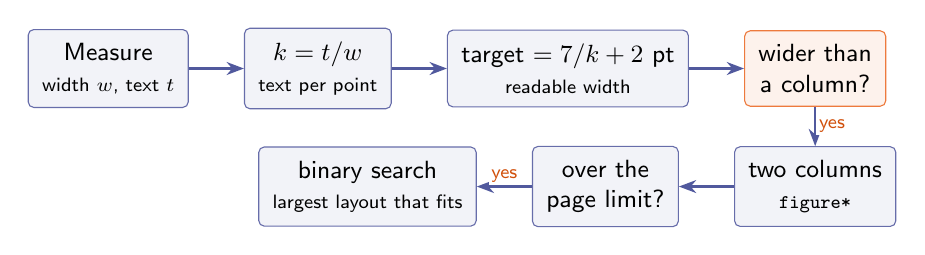
\begin{tikzpicture}[node distance=5mm and 7mm]
\node[blk] (a) {Measure\\\scriptsize width $w$, text $t$};
\node[blk, right=of a] (b) {$k = t / w$\\\scriptsize text per point};
\node[blk, right=of b] (c) {target $= 7/k + 2$ pt\\\scriptsize readable width};
\node[hot, right=of c] (d) {wider than\\a column?};
\node[blk, below=of d] (e) {two columns\\\scriptsize \code{figure*}};
\node[blk, left=of e] (f) {over the\\page limit?};
\node[blk, left=of f] (g) {binary search\\\scriptsize largest layout that fits};
\draw[arr] (a)--(b); \draw[arr] (b)--(c); \draw[arr] (c)--(d);
\draw[arr] (d)--node[lab,right]{yes}(e); \draw[arr] (e)--(f); \draw[arr] (f)--node[lab,above]{yes}(g);
\end{tikzpicture}
\caption{The figure fitter. If even the smallest readable layout is over the limit, Prarup reports how many
pages to cut instead of making text unreadable, or offers a second layout and lets the author choose.}
\end{figure}

On the damaged SVM paper used in Chapter~\ref{ch:eval}, two figures printed their text at 3.9~pt. The fitter
moved both to two-column figures, measured their text at 7.0~pt afterwards, and the paper stayed at six
pages (Table~\ref{tab:fit}).

\begin{table}[htbp]
\centering\small
\caption{Figure fitter output on the damaged SVM paper, as printed in the Figure fit tab.}
\label{tab:fit}
\begin{tabular}{l l l l}
\toprule
Figure & Before & After & Note\\
\midrule
Fig. 3 & 3.42 in, one column, 7.3 pt & unchanged & already readable\\
Fig. 4 & 3.42 in, one column, 3.9 pt & 6.13 in, both columns, 7.0 pt & resized\\
Fig. 5 & 3.42 in, one column, 3.9 pt & 6.13 in, both columns, 7.0 pt & resized\\
Fig. 1 & 3.42 in & unchanged & no text to measure\\
\midrule
\multicolumn{4}{l}{Pages: 6 \textrightarrow{} 6, limit 6}\\
\bottomrule
\end{tabular}
\end{table}

\section{The desktop window}
The window has the outline of the paper on the left, an editor for the chosen block in the middle with
five tabs below it, and the PDF on the right (Figure~\ref{fig:ui}). Rows with a problem are red and marked
with a warning sign; clicking a problem in a tab opens its block.

\begin{figure}[htbp]
\centering
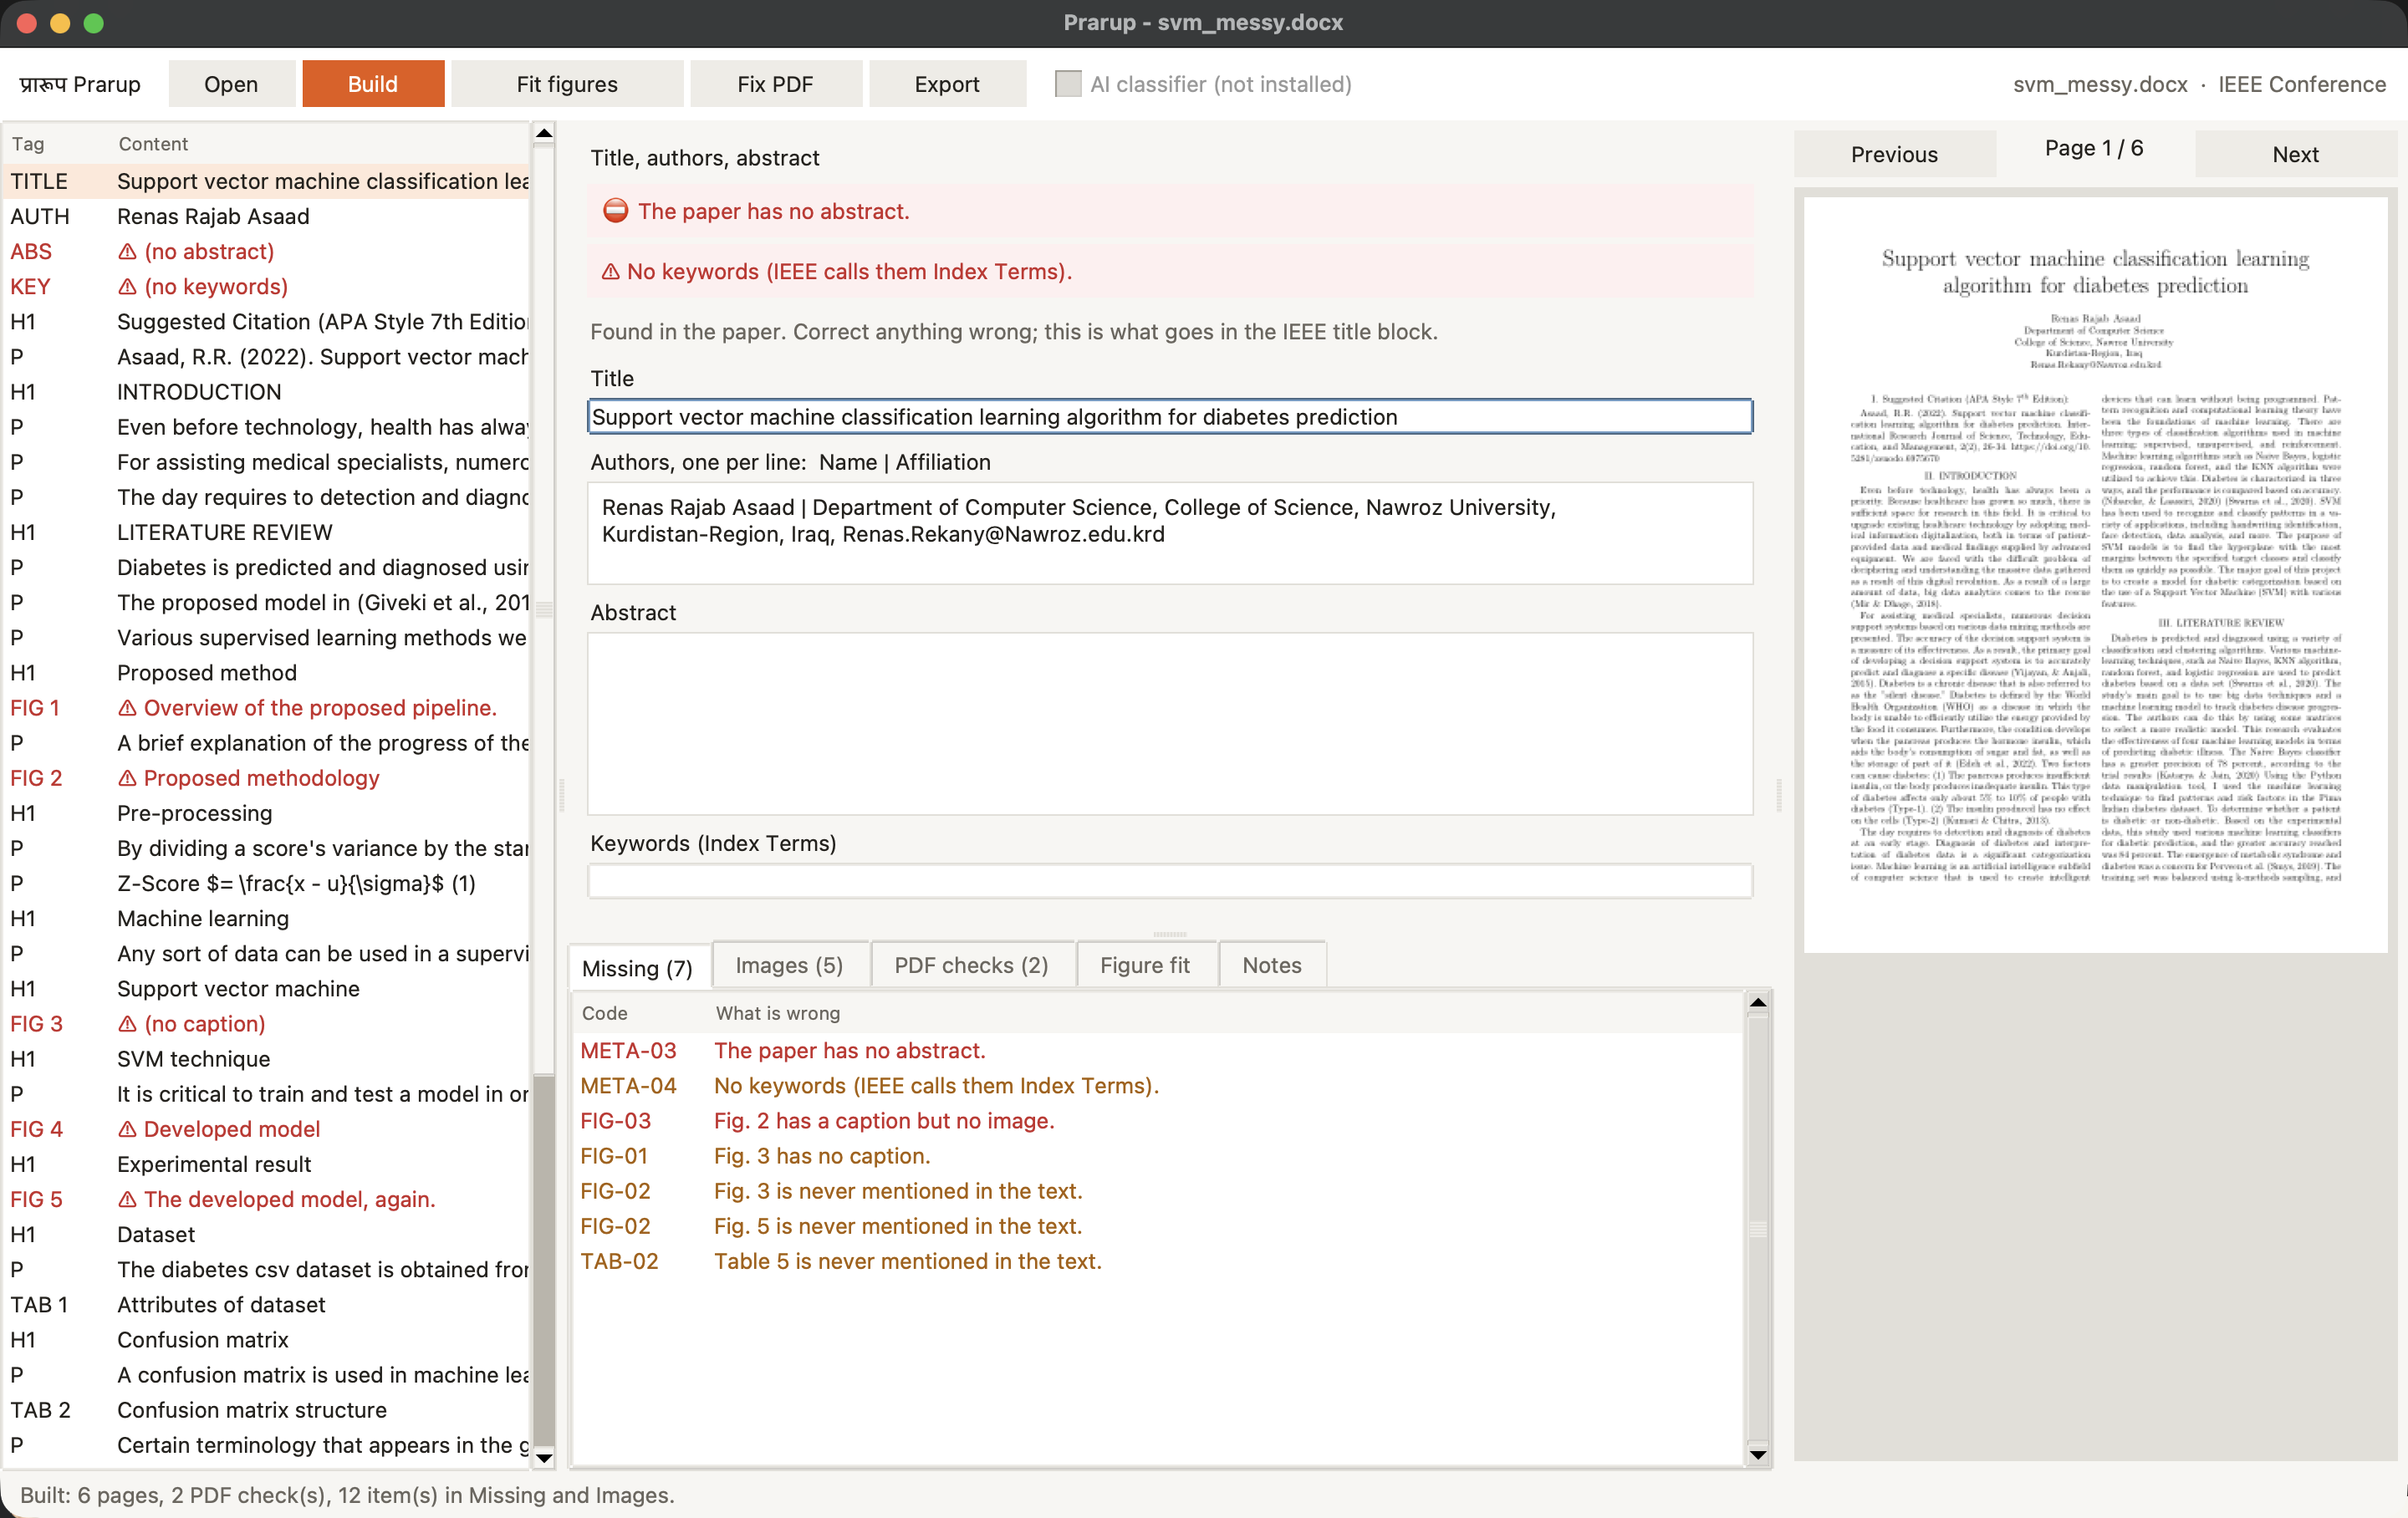
\includegraphics[width=\linewidth]{fig/ui-opened.png}
\caption{The damaged SVM paper just after opening. The Missing tab lists seven items; the outline marks the
missing abstract and keywords and the figure without a caption.}
\label{fig:ui}
\end{figure}

Building takes several seconds, so it runs on one background thread. Tkinter is not thread-safe: only the
main thread may touch a widget. The background thread therefore only computes and returns a result, and the
main thread checks every 80~ms, using Tk's own timer, whether the result is ready and then draws it. After
an edit the build is scheduled 1.5~seconds later, and a further edit restarts the timer, so typing does not
start a build per keystroke.

\begin{figure}[htbp]
\centering
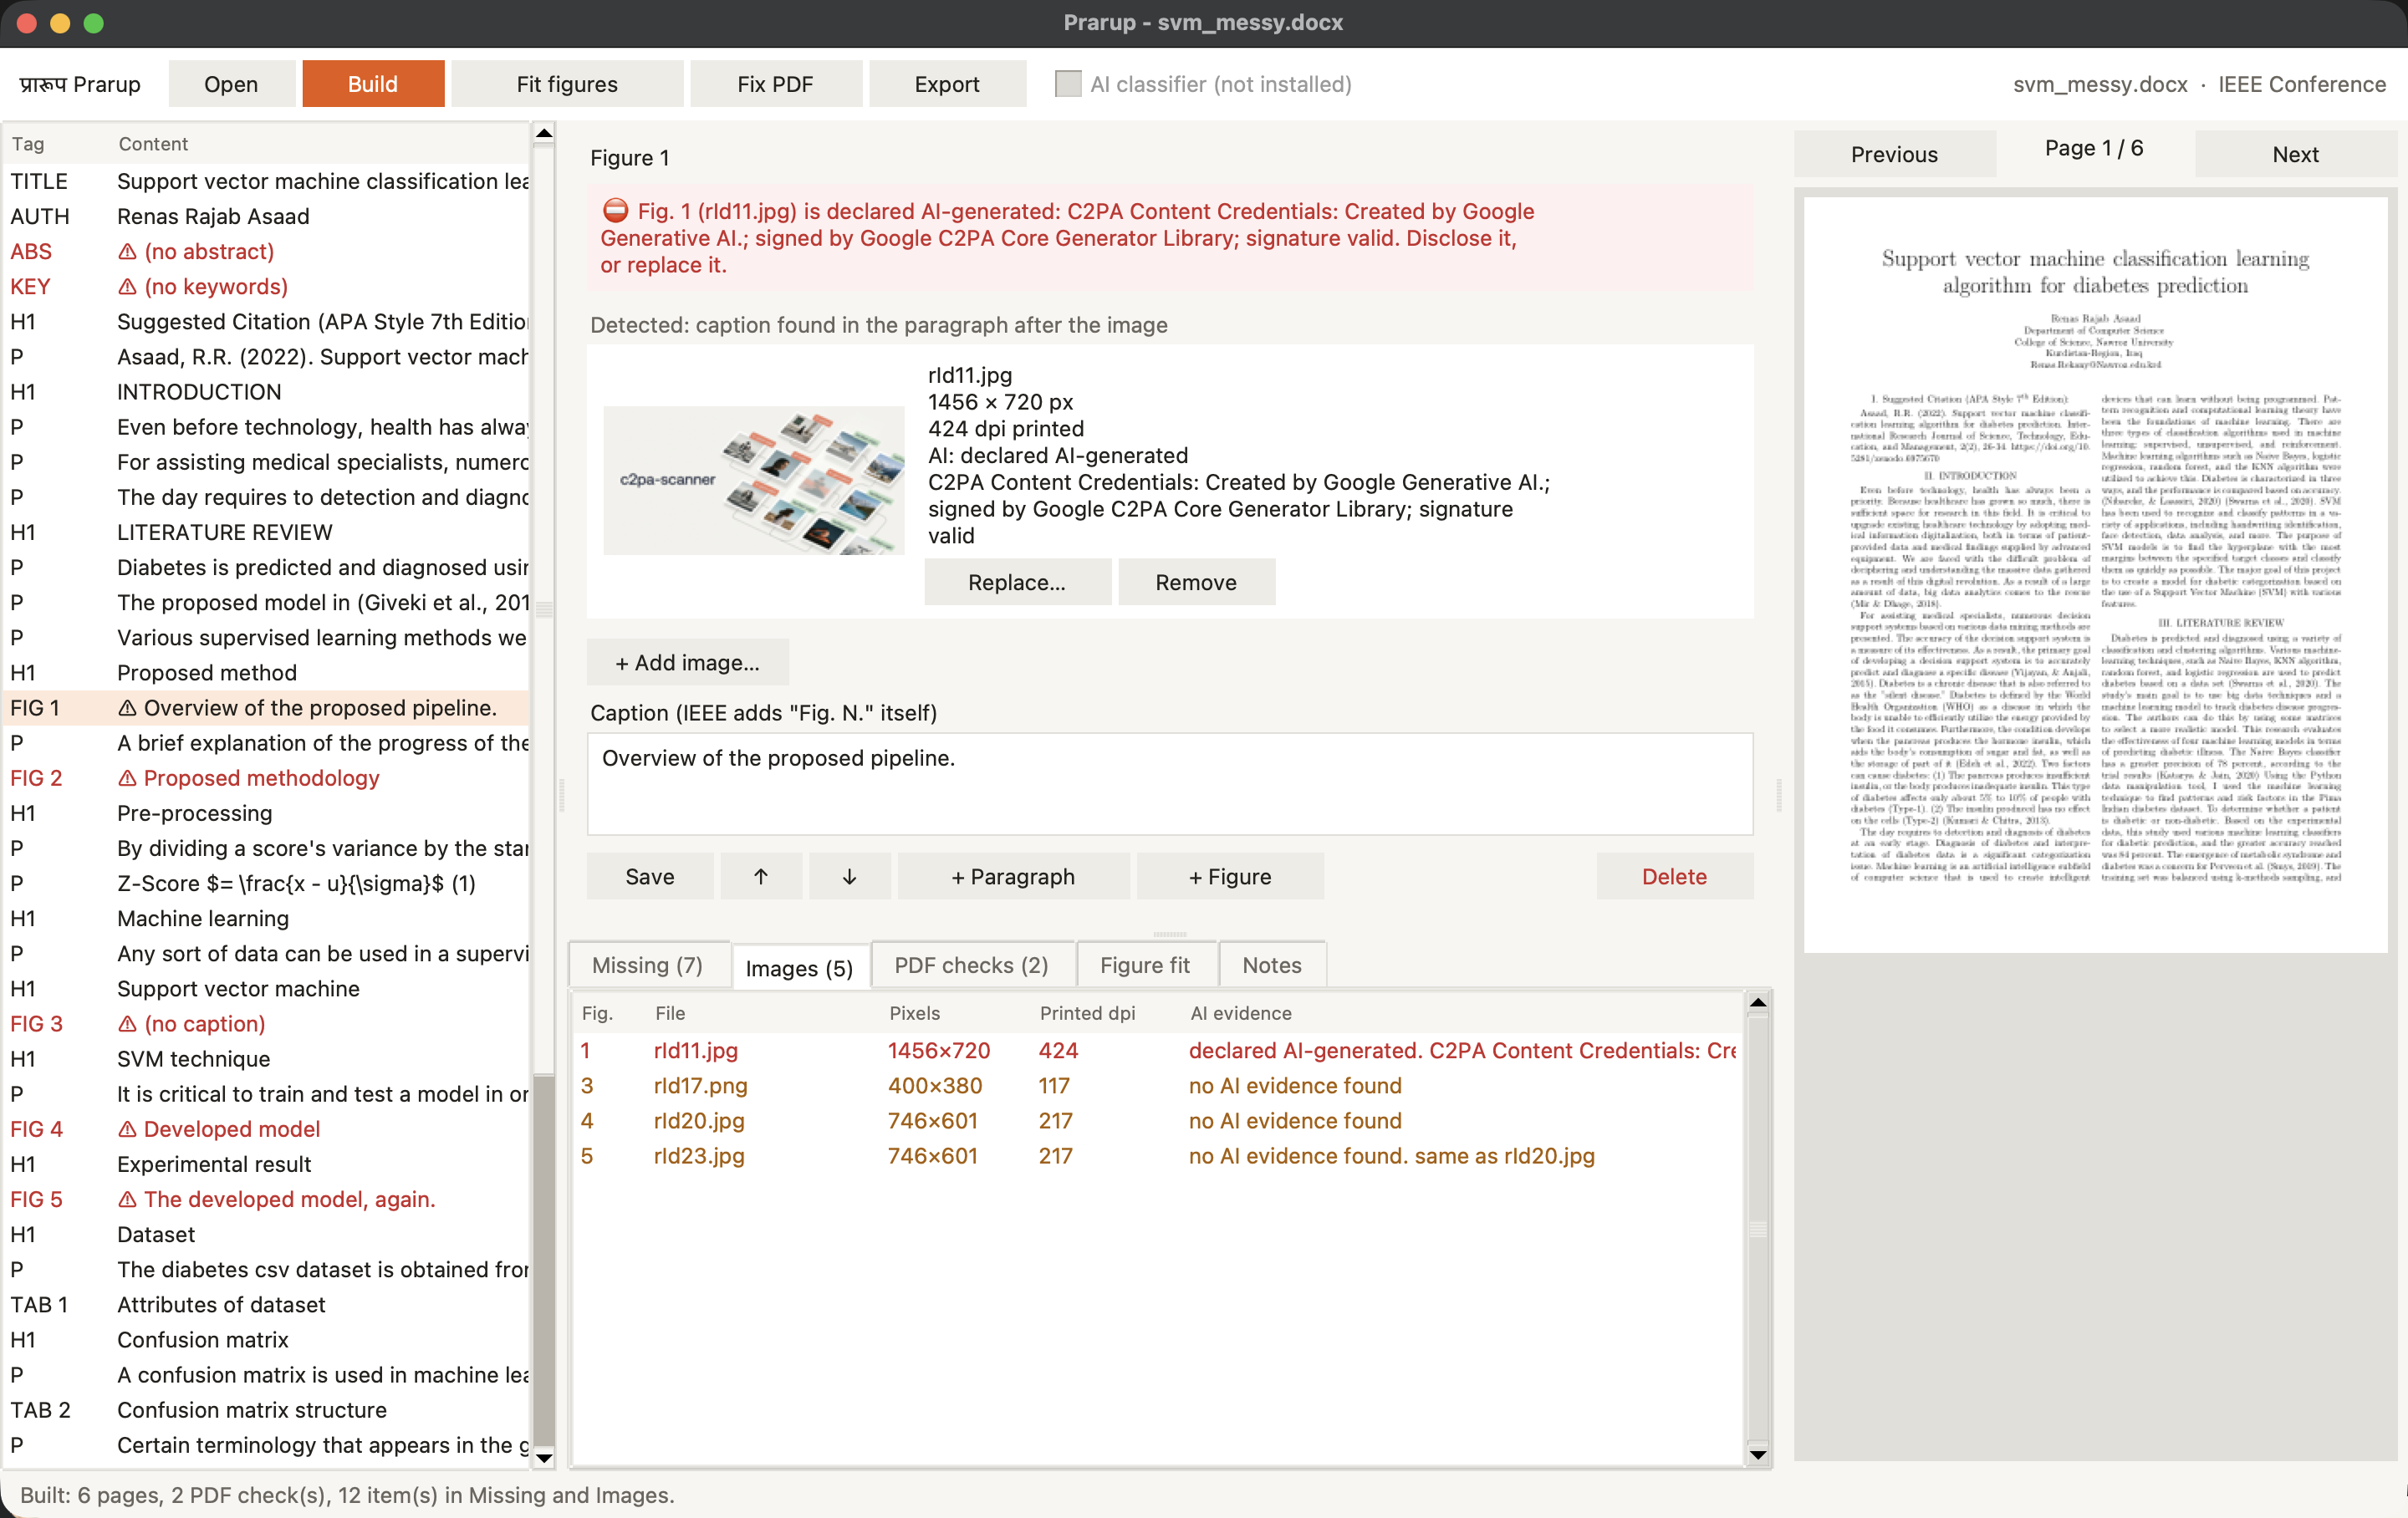
\includegraphics[width=\linewidth]{fig/ui-ai.png}
\caption{The figure editor on the AI-generated image planted in the paper. Google's signed C2PA record is
read and shown; the Images tab lists every image with its pixels, printed dpi and AI evidence.}
\label{fig:uiai}
\end{figure}

\begin{figure}[htbp]
\centering
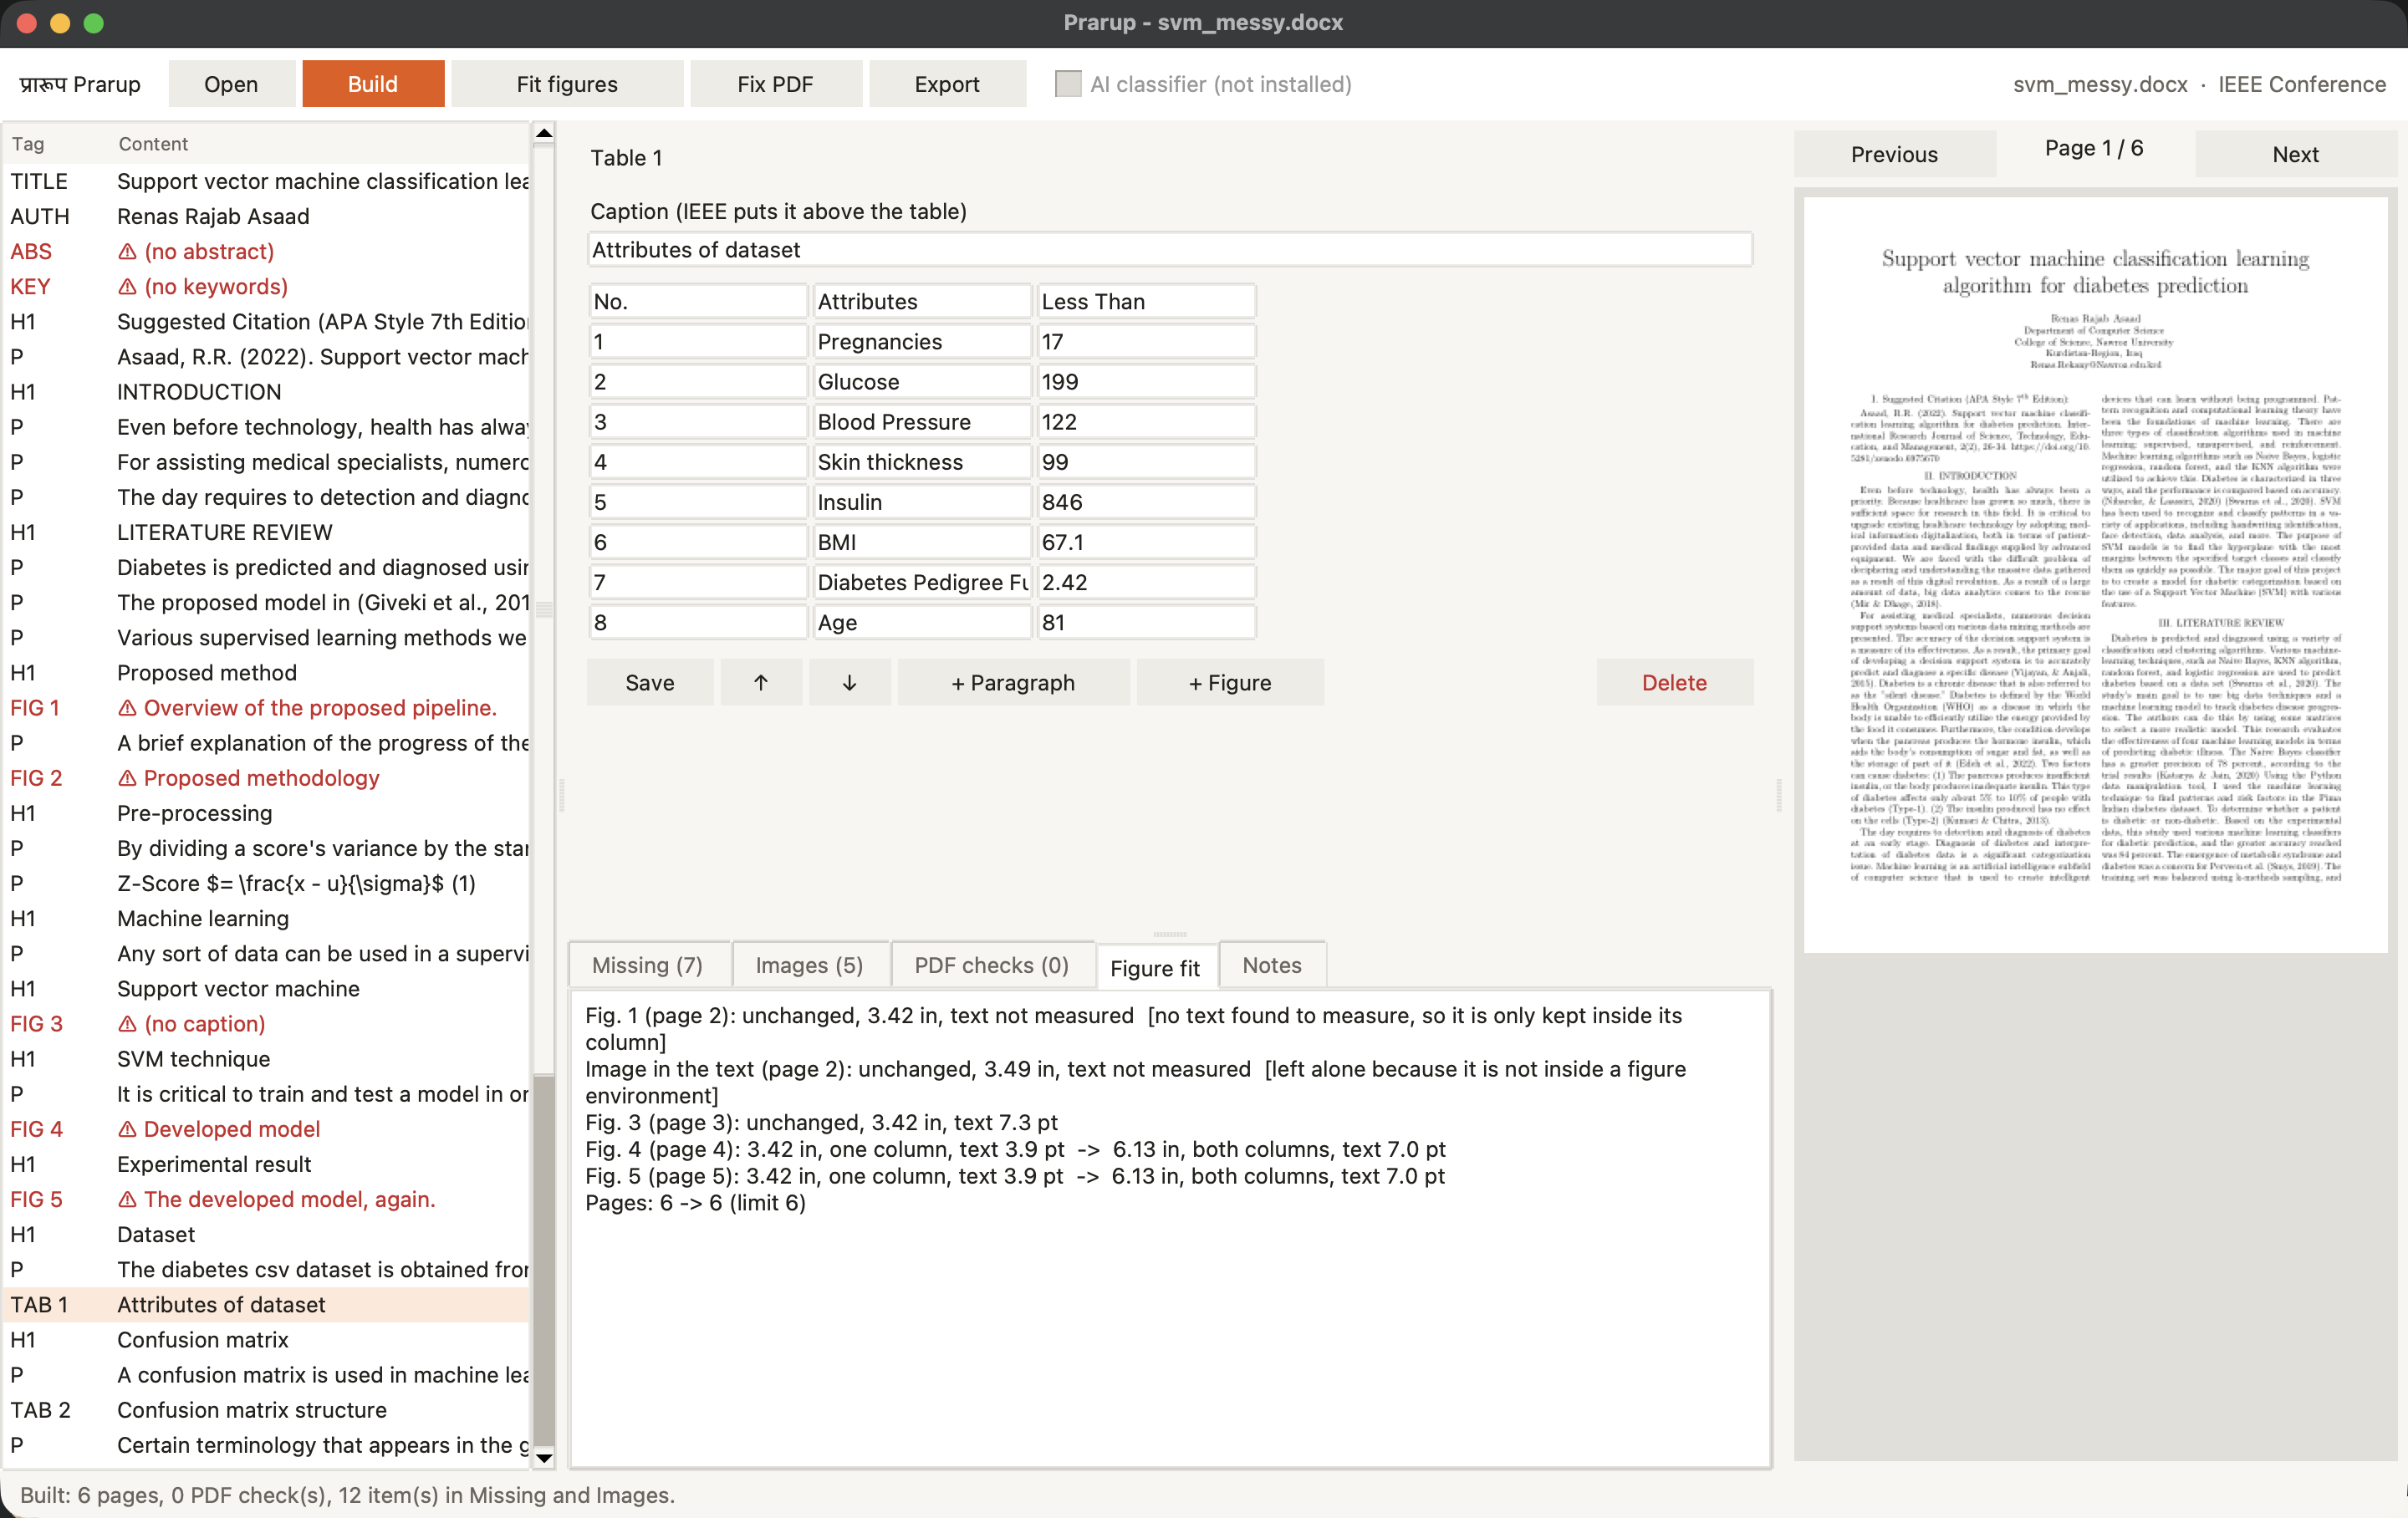
\includegraphics[width=\linewidth]{fig/ui-fit.png}
\caption{After Fit figures. The Figure fit tab reports each figure before and after; two figures moved from
3.9~pt to 7.0~pt text.}
\end{figure}

Each kind of block has its own editor: the title block, text blocks (which can be re-tagged as heading,
paragraph or quote), figures (image cards with Replace and Remove), tables (a grid of cells written back
into the document tree) and references. Every editor's \code{save()} writes through the controller and
returns a message; it never redraws the window itself. Our first version did, and crashed when an editor
destroyed itself in the middle of saving.

\section{Export}
Export builds the paper once more and writes a zip archive containing the PDF, the generated \LaTeX, every
image the \LaTeX{} uses, the bibliography file if there is one, a Markdown report of every check, and a
short README explaining how to compile it.

% ---------------------------------------------------------------- 6
\chapter{Evaluation}\label{ch:eval}

\begin{takeaway}
We tested on real papers rather than examples we wrote ourselves, then damaged copies of them on purpose
so that every check had something real to find. All six real papers now compile, and every planted fault
is detected and repaired through the window.
\end{takeaway}

\section{Test material}
\begin{itemize}
\item \textbf{Three Word papers} from Zenodo under CC BY 4.0, on football analytics, UAV imagery and
diabetes prediction~\cite{zyolo,zuav,zsvm}. They are included in the repository as test fixtures.
\item \textbf{Three \LaTeX{} papers} from arXiv, two with \code{.bib} files and one split across six
\code{\textbackslash input} files. Their licence does not allow redistribution, so the repository contains a small
\LaTeX{} project of our own that reproduces every construct they broke on.
\item \textbf{Four real AI images}: one signed by Google's Gemini with C2PA, one Stable Diffusion image with its
settings intact, and two generated images with their metadata removed.
\item \textbf{Damaged papers} made by a script, \code{tools/make\_messy.py}, which edits the real papers'
document trees: deleting captions, the abstract and keywords, shrinking an image to 400 pixels, inserting
the Gemini image byte for byte, duplicating a figure, and citing [99] in a paper with 50 references.
\end{itemize}

\section{Results}

\begin{figure}[htbp]
\centering
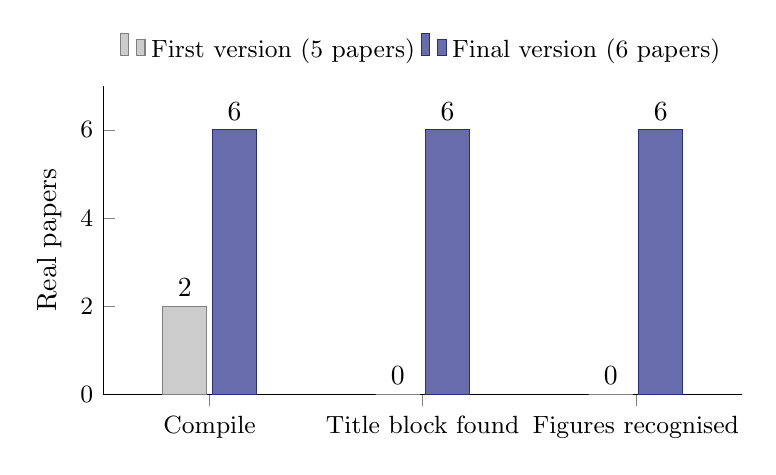
\begin{tikzpicture}
\begin{axis}[ybar, bar width=16pt, ymin=0, ymax=7, ylabel={Real papers}, width=0.8\linewidth, height=55mm,
  symbolic x coords={Compile, Title block found, Figures recognised}, xtick=data,
  nodes near coords, legend style={at={(0.5,1.04)},anchor=south,legend columns=2,draw=none,font=\small},
  enlarge x limits=0.25, axis lines*=left, ticklabel style={font=\small}]
\addplot[fill=gray!40, draw=gray] coordinates {(Compile,2) (Title block found,0) (Figures recognised,0)};
\addplot[fill=dau!70, draw=dau] coordinates {(Compile,6) (Title block found,6) (Figures recognised,6)};
\legend{First version (5 papers), Final version (6 papers)}
\end{axis}
\end{tikzpicture}
\caption{Real papers before and after the redesign. The first version typed the title block by hand and
did not recognise figures at all.}
\end{figure}

\begin{table}[htbp]
\centering\small
\caption{Planted faults in the damaged SVM paper, and whether Prarup found and repaired each one through the window.}
\begin{tabularx}{\linewidth}{X l c c}
\toprule
Fault planted & Finding & Found & Repaired\\
\midrule
Abstract deleted & META-03 & yes & yes, title-block editor\\
Keywords deleted & META-04 & yes & yes\\
Caption of a figure deleted & FIG-01 & yes & yes, figure editor\\
Image shrunk to 400 px & IMG-01, 117 dpi & yes & yes, image replaced\\
Gemini image inserted & IMG-02, C2PA & yes & yes, image replaced\\
A figure duplicated & IMG-05 & yes & yes, block deleted\\
Figure whose image was lost & FIG-03 & yes & yes, image added\\
\bottomrule
\end{tabularx}
\end{table}

The same holds for the damaged UAV paper (a deleted caption and keywords, and a citation of [99] against 50
references, found as REF-02) and for the zipped \LaTeX{} project (a deleted caption, a 70~dpi copy of a plot,
a duplicate, a citation of an unknown key and a missing image). Testing on damaged papers also found three
bugs in Prarup itself, which we fixed: a citation like [99] was not checked in papers that also used
author-year citations, the abstract was not searched for citations, and clicking that finding opened the
title instead of the paragraph.

\begin{figure}[htbp]
\centering
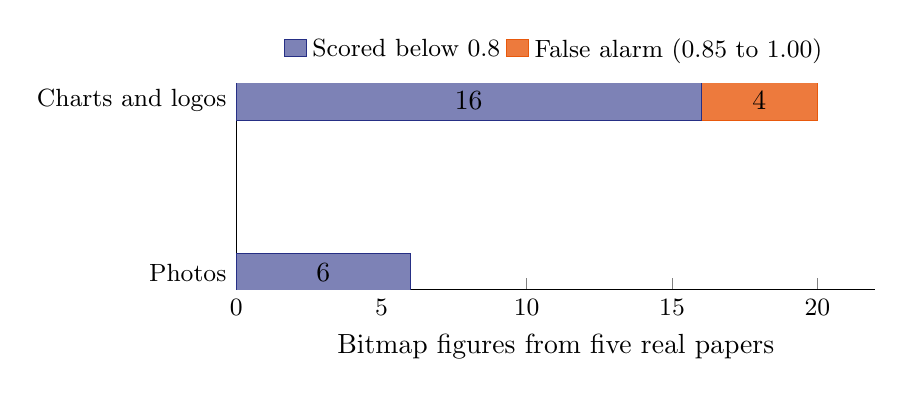
\begin{tikzpicture}
\begin{axis}[xbar stacked, bar width=14pt, xmin=0, xmax=22, width=0.8\linewidth, height=42mm,
  symbolic y coords={Photos, Charts and logos}, ytick=data, xlabel={Bitmap figures from five real papers},
  legend style={at={(0.5,1.05)},anchor=south,legend columns=2,draw=none,font=\small}, axis lines*=left,
  nodes near coords, ticklabel style={font=\small}]
\addplot[fill=dau!60,draw=dau] coordinates {(16,Charts and logos) (6,Photos)};
\addplot[fill=dauorange!80,draw=dauorange] coordinates {(4,Charts and logos) (0,Photos)};
\legend{Scored below 0.8, False alarm (0.85 to 1.00)}
\end{axis}
\end{tikzpicture}
\caption{The optional AI classifier on 26 real, human-made figures. All four false alarms were charts or
logos, which is why the classifier now runs only on photo-like images. All four real AI images scored 1.00.}
\end{figure}

\paragraph{AI evidence on real AI images}
The Gemini image was reported as declared AI-generated, with Google's signature validated. The Stable
Diffusion image was reported through its generation settings (30 steps, Euler a sampler). The two images
with stripped metadata showed no metadata evidence, which is the correct and honest result; only the
classifier, when installed, detected them.

\paragraph{Automated tests}
The repository has 147 automated tests written with pytest. They cover each module on the real fixtures,
the compiled PDFs, the image checks on the real AI images, and the window itself, which a test drives
through opening the damaged SVM paper, clicking a problem, typing the missing text, replacing images,
deleting the duplicate, building and exporting. Tests that need a program which is not installed are
skipped rather than failed.

% ---------------------------------------------------------------- 7
\chapter{Discussion}\label{ch:disc}

\begin{takeaway}
The main lesson was that real documents are messier than any example we would have written, and that the
honest answer to an uncertain question is evidence with its strength attached.
\end{takeaway}

\section{What we learned}
Our first design compiled the author's own \LaTeX{} and asked the user to type the title and authors. It
worked on our examples and failed on most real papers. Testing early on real files changed the design
more than any planning did: the decision to rebuild every paper in our own template came directly from
watching real Word tables and arXiv preambles break. The same experience made us measure the AI classifier
before trusting it, and the measurement reversed our plan to run it on every image.

A second lesson concerned the window. We rewrote it twice, first from a web prototype to PySide6, then from
PySide6 to Tkinter, after a team member showed that a smaller window was easier to understand and explain.
Moving the work into a controller class made both rewrites cheap: the window is only a quarter of the code,
and none of the checks had to change.

\section{Limitations}
\begin{itemize}
\item Only the IEEE conference template is supported.
\item Author detection covers the layouts we found in our test papers; an unusual layout may put a name in
the wrong field, which the title-block editor shows so it can be corrected.
\item OCR text size is accurate to about half a point on clean plots; dense screenshots read lower.
\item An AI image with its metadata removed can only be caught by the optional classifier, which gives a
likelihood, not proof.
\item \LaTeX{} constructs that pandoc cannot read appear as raw blocks, and packages that change page layout
are deliberately not carried over.
\end{itemize}

% ---------------------------------------------------------------- 8
\chapter{Conclusion and future work}\label{ch:conc}

Prarup turns the publisher's late, unexplained rejection into an early, located and mostly repairable list
of problems. It reads both formats researchers use into one editable structure, checks what is missing,
measures figures on the page and makes their text readable, reports AI-image evidence honestly, and builds
a PDF that passes the checks IEEE applies. Every result in this report can be reproduced from the
repository with one command.

The natural next steps are other templates (ACM and Springer, through new template and rule files),
PDF/A output for archiving, margin checks, and clicking a point in the PDF to jump to the block that produced
it, using the SyncTeX data the build already writes.

\appendix
\chapter{Running Prarup}
\begin{lstlisting}[language=bash]
pip install -r requirements.txt          # Python libraries
# install pandoc, tectonic and ghostscript (tesseract optional)
python -m prarup.main paper.docx          # open the window on a paper
python -m pytest                          # run the 147 tests
pip install -r requirements-ai.txt        # optional AI classifier
\end{lstlisting}
The source code, tests, test papers and this report are in the repository
\url{https://github.com/Krushna-007/prarup}.

\backmatter
\begin{thebibliography}{99}
\small
\bibitem{minto} B. Minto, \emph{The Pyramid Principle: Logic in Writing and Thinking}, 3rd ed. Pearson, 2009.
\bibitem{gopen} G. D. Gopen and J. A. Swan, ``The science of scientific writing,'' \emph{American Scientist}, vol. 78, no. 6, pp. 550--558, 1990.
\bibitem{pinker} S. Pinker, \emph{The Sense of Style: The Thinking Person's Guide to Writing in the 21st Century}. Viking, 2014.
\bibitem{pdfexpress} IEEE, ``IEEE PDF eXpress,'' \url{https://ieee-pdf-express.org}.
\bibitem{ieeetran} M. Shell, ``How to use the IEEEtran \LaTeX{} class,'' IEEE, 2015.
\bibitem{ieeegraphics} IEEE Author Center, ``Preparing figures and graphics,'' \url{https://journals.ieeeauthorcenter.ieee.org}.
\bibitem{pandoc} J. MacFarlane, ``Pandoc: a universal document converter,'' \url{https://pandoc.org}.
\bibitem{tectonic} The Tectonic Project, ``Tectonic: a modernized \TeX/\LaTeX{} engine,'' \url{https://tectonic-typesetting.github.io}.
\bibitem{pymupdf} Artifex, ``PyMuPDF documentation,'' \url{https://pymupdf.readthedocs.io}.
\bibitem{ghostscript} Artifex, ``Ghostscript,'' \url{https://www.ghostscript.com}.
\bibitem{tesseract} R. Smith, ``An overview of the Tesseract OCR engine,'' in \emph{Proc. ICDAR}, 2007, pp. 629--633.
\bibitem{c2pa} Coalition for Content Provenance and Authenticity, ``C2PA technical specification,'' \url{https://c2pa.org/specifications}.
\bibitem{iptc} IPTC, ``Digital source type vocabulary,'' \url{https://cv.iptc.org/newscodes/digitalsourcetype}.
\bibitem{dhash} N. Krawetz, ``Kind of like that,'' The Hacker Factor Blog, 2013 (difference hash).
\bibitem{aiclassifier} Ateeqq, ``ai-vs-human-image-detector,'' Hugging Face model, \url{https://huggingface.co/Ateeqq/ai-vs-human-image-detector}.
\bibitem{zyolo} Roy, ``YOLO-based football analysis,'' Zenodo 16929566, CC BY 4.0.
\bibitem{zuav} Sharp \emph{et al.}, ``Machine learning for UAV and ground imagery,'' Zenodo 11105119, CC BY 4.0.
\bibitem{zsvm} R. R. Asaad, ``Support vector machine classification learning algorithm for diabetes prediction,'' Zenodo 6975670, CC BY 4.0.
\end{thebibliography}

\noindent\footnotesize Page layout modelled on the Hagenberg Thesis document class by W. Burger and W.
Hochleitner (CC BY 4.0).
\end{document}
